\begin{figure}[p]
    \centering
    \begin{subfigure}{0.47\linewidth}
        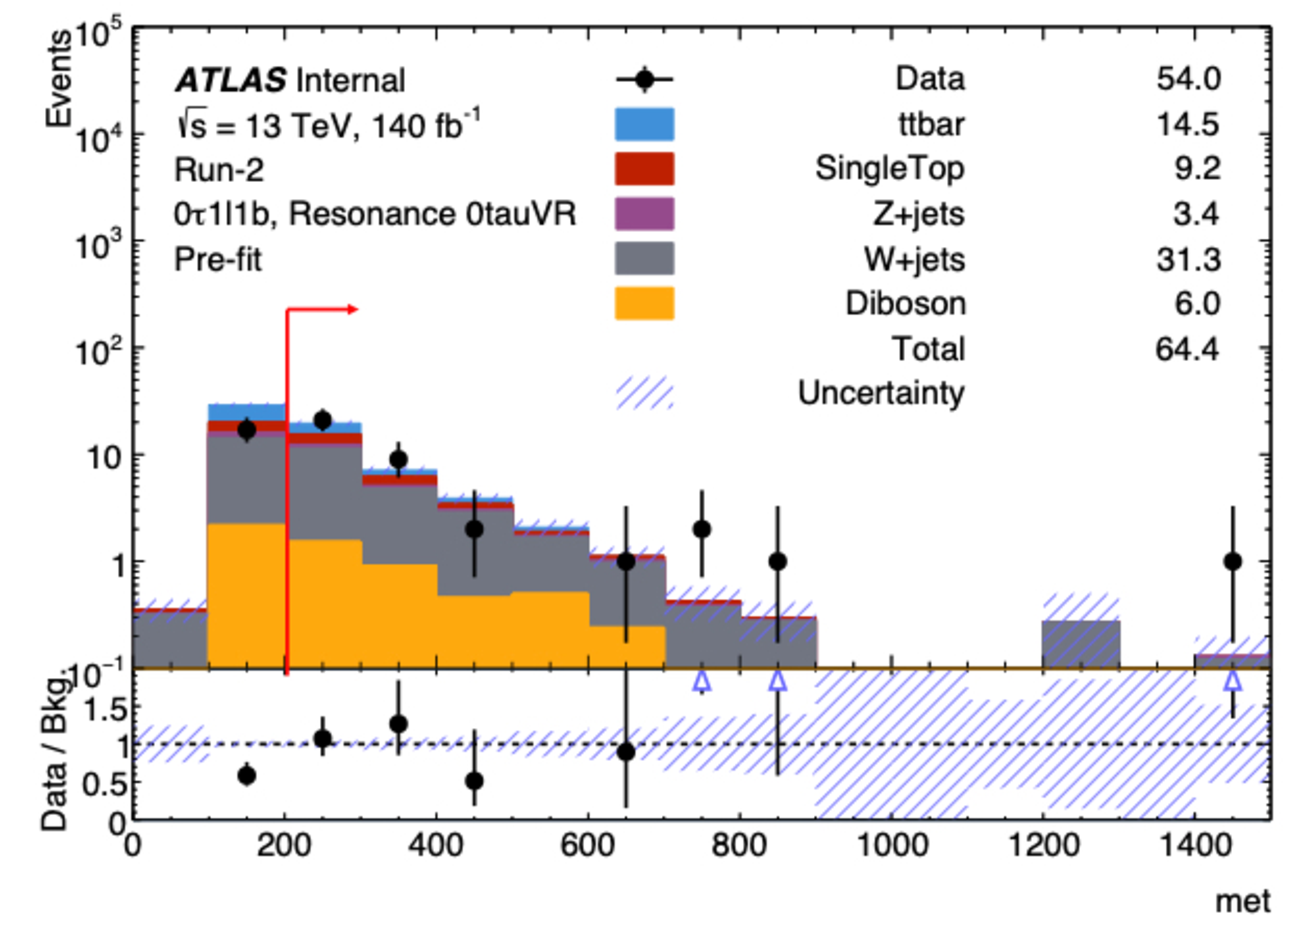
\includegraphics[width=\linewidth]{Figs/CH8/VRW_Res_met.pdf}
        \caption[]{$\met$}
    \end{subfigure}\hfill
    \begin{subfigure}{0.47\linewidth}
        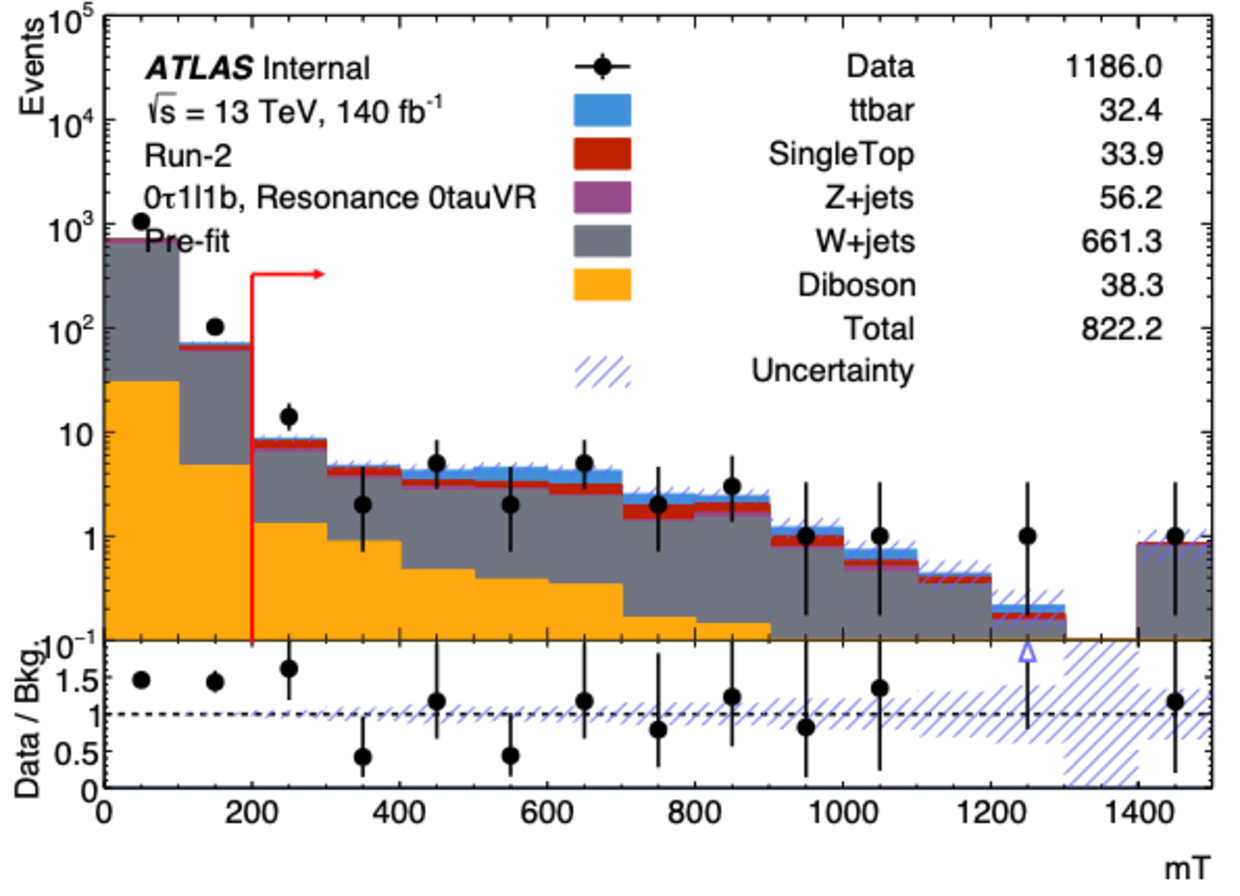
\includegraphics[width=\linewidth]{Figs/CH8/VRW_Res_mT.pdf}
        \caption[]{$\mT^\ell$}
    \end{subfigure}\par\medskip
    \begin{subfigure}{0.47\linewidth}
        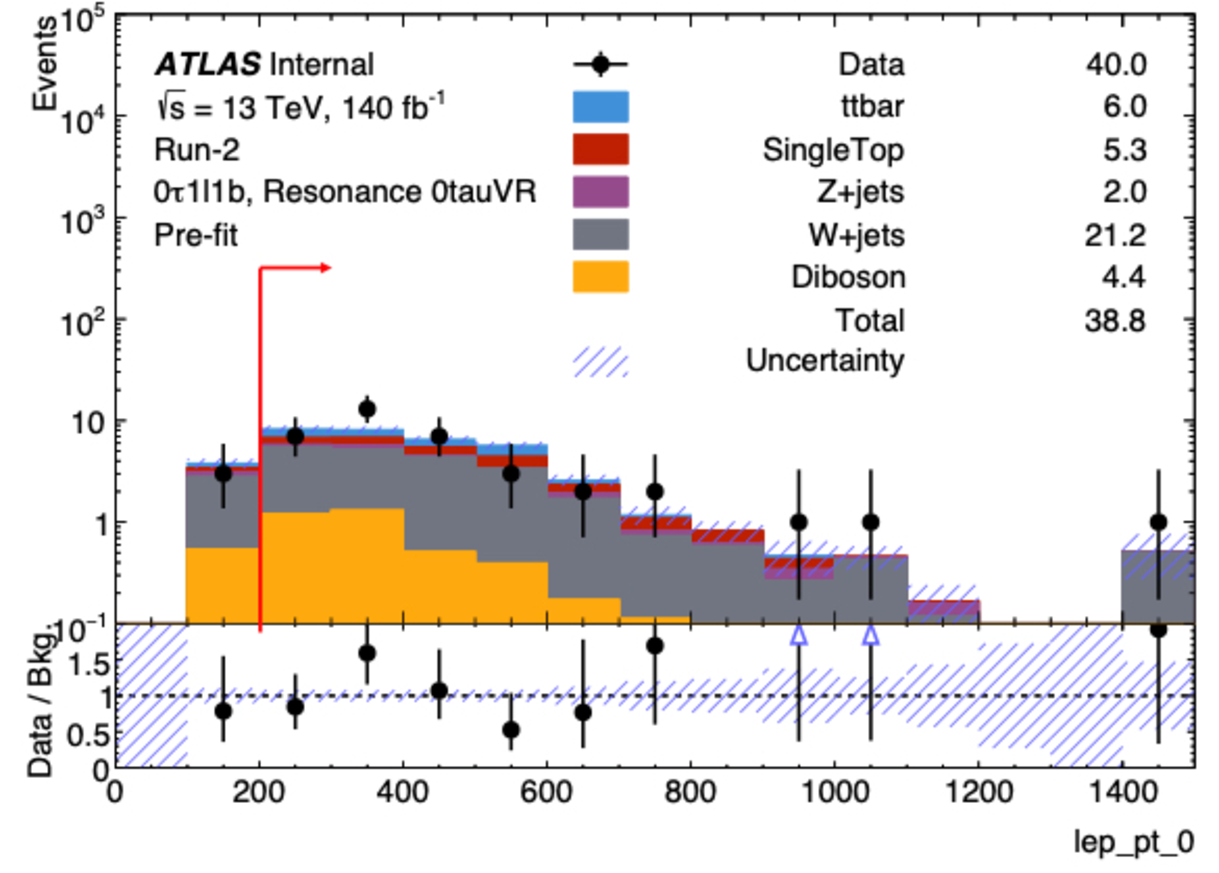
\includegraphics[width=\linewidth]{Figs/CH8/VRW_Res_lep_pT.pdf}
        \caption[]{$\pT^\ell$}
    \end{subfigure}\hfill
    \begin{subfigure}{0.47\linewidth}
        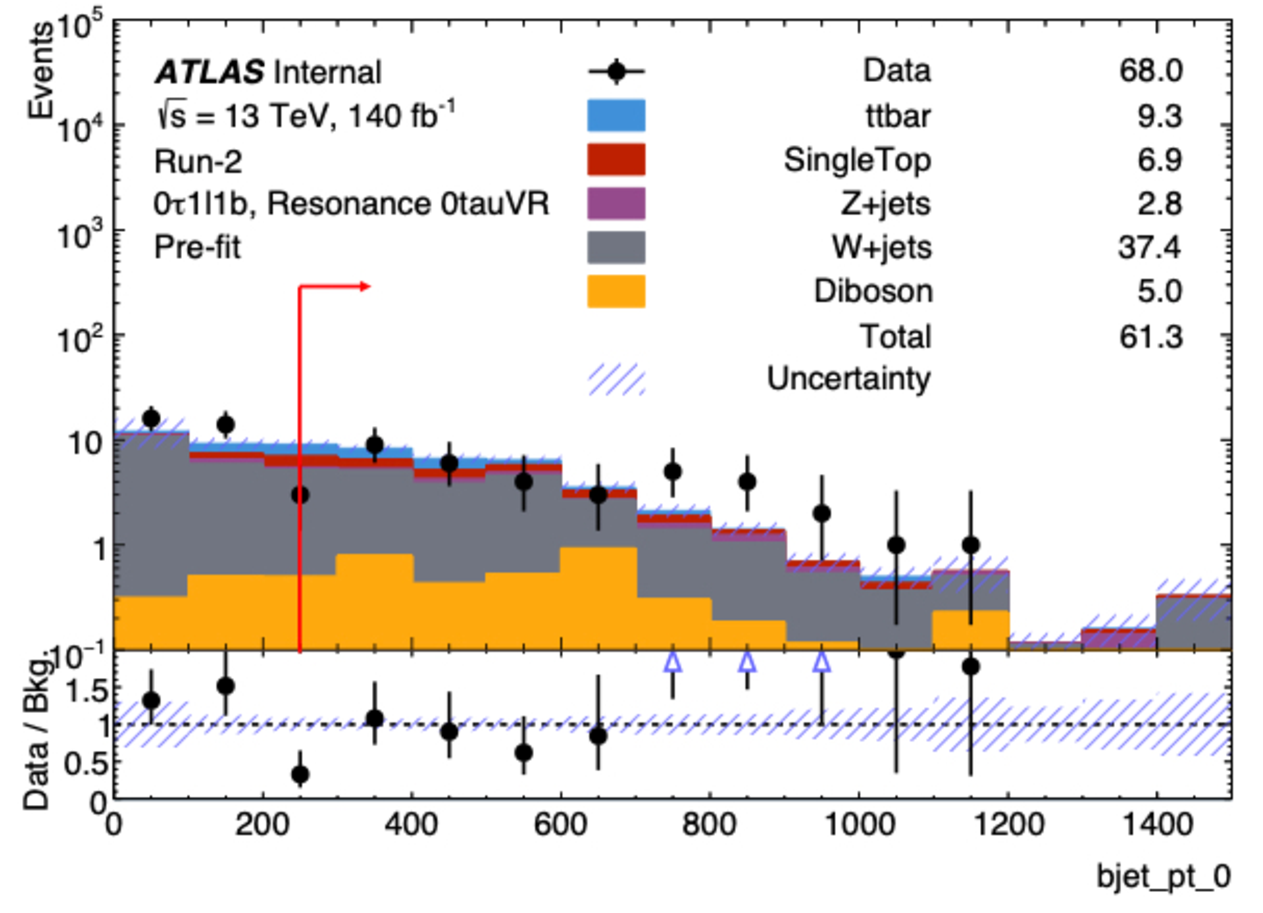
\includegraphics[width=\linewidth]{Figs/CH8/VRW_Res_b_pT.pdf}
        \caption[]{$\pT^b$}
    \end{subfigure}\par\medskip
    \begin{subfigure}{0.47\linewidth}
        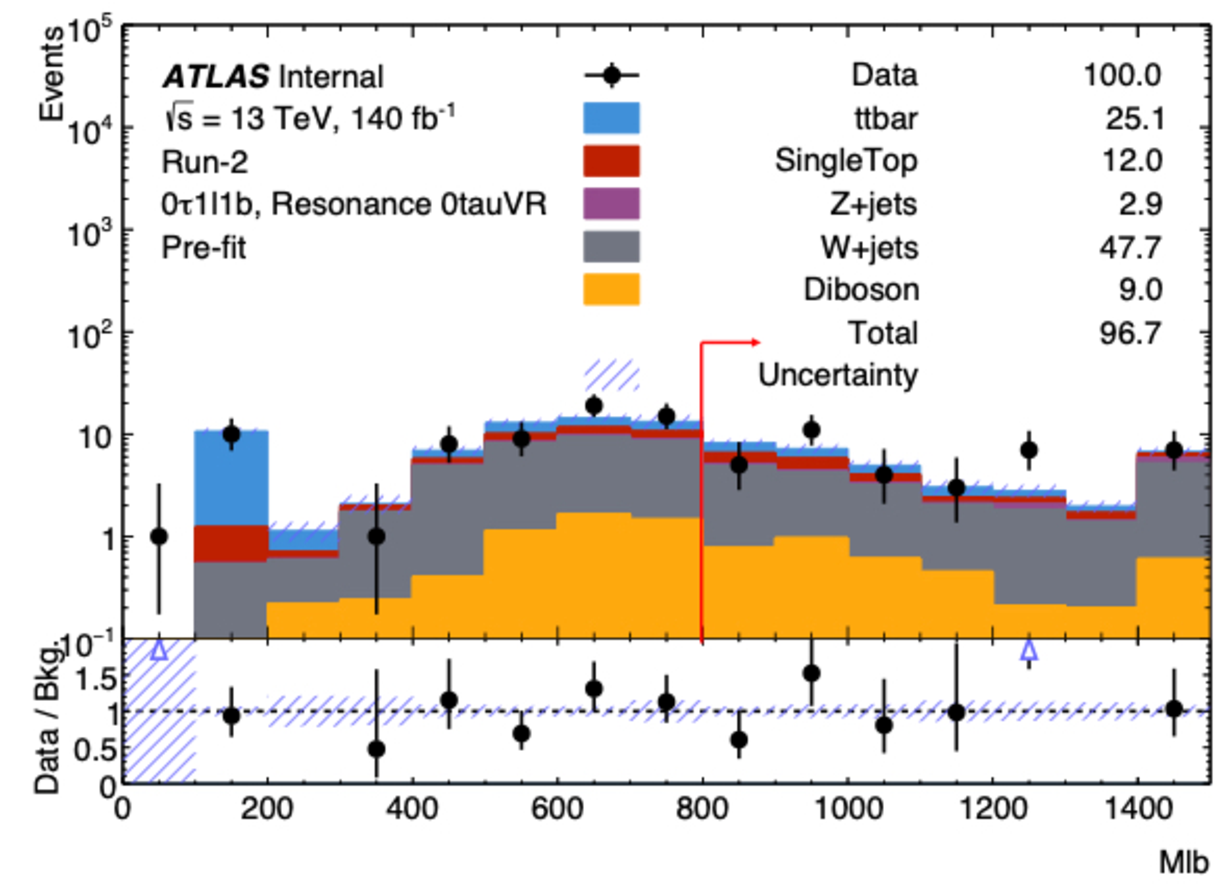
\includegraphics[width=\linewidth]{Figs/CH8/VRW_Res_Mlb.pdf}
        \caption[]{$m_{b\ell}$}
    \end{subfigure}\hfill
    \begin{subfigure}{0.47\linewidth}
        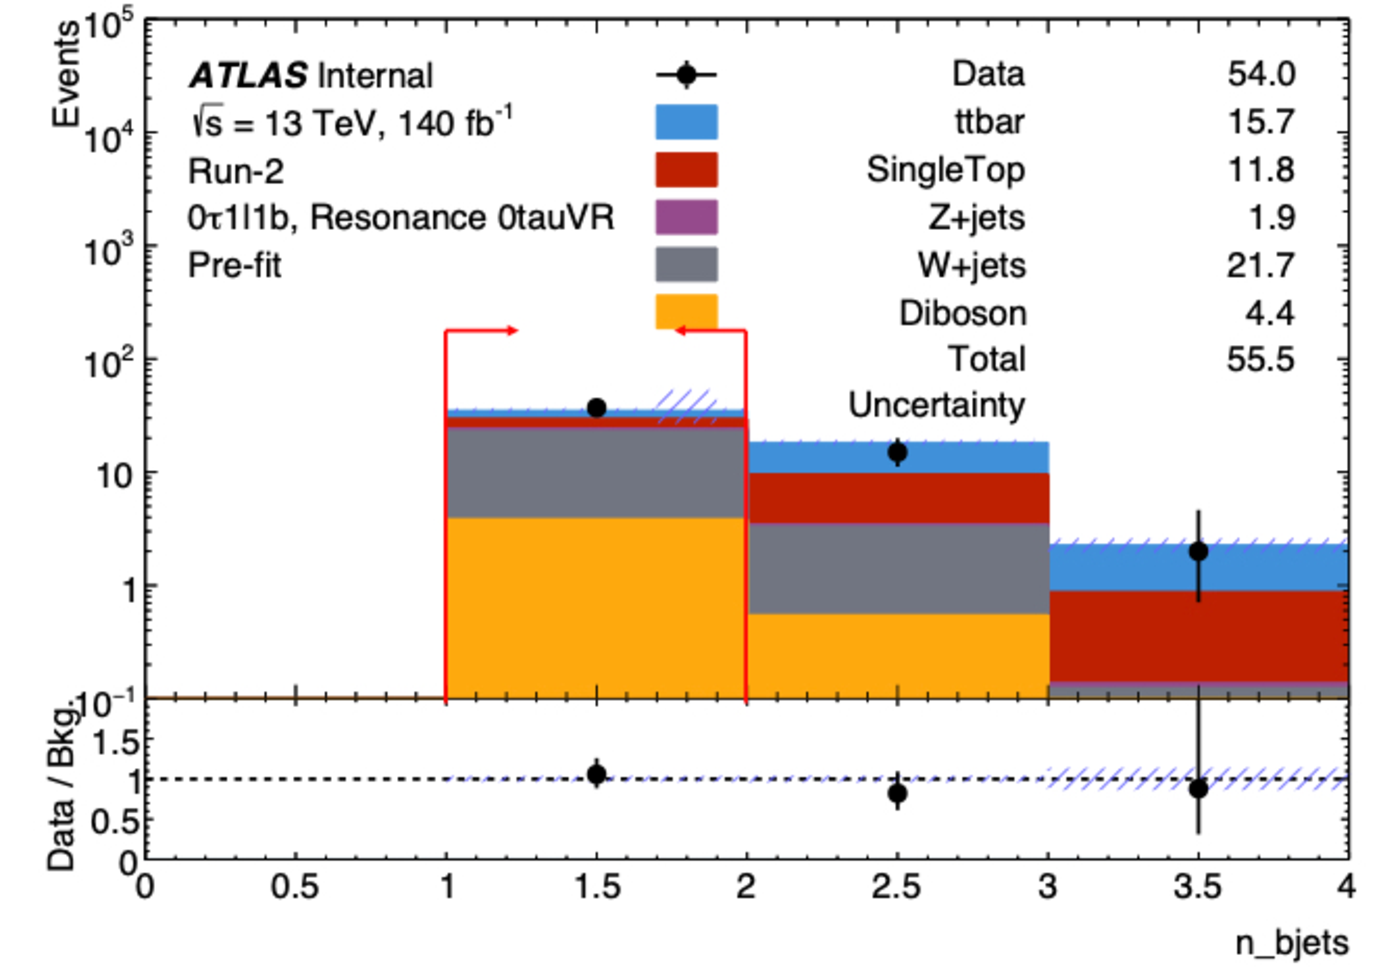
\includegraphics[width=\linewidth]{Figs/CH8/VRW_Res_nbjets.pdf}
        \caption[]{$N_b$}
    \end{subfigure}\par\medskip
    \caption[Pre-fit N-1 distributions in VRW-Res]{Pre-fit $N-1$ distributions in VRW-Res. The electron and muon channels are combined. The lower panels show data divided by the total simulated background. The hatched bands represent the statistical uncertainty in the prediction. The last bin includes the overflow. The original plot labels $0\tau$VR denote $\VRb$.}
    \label{fig:ch8_vrw_res}
\end{figure}

\begin{figure}[p]
    \centering
    \begin{subfigure}{0.47\linewidth}
        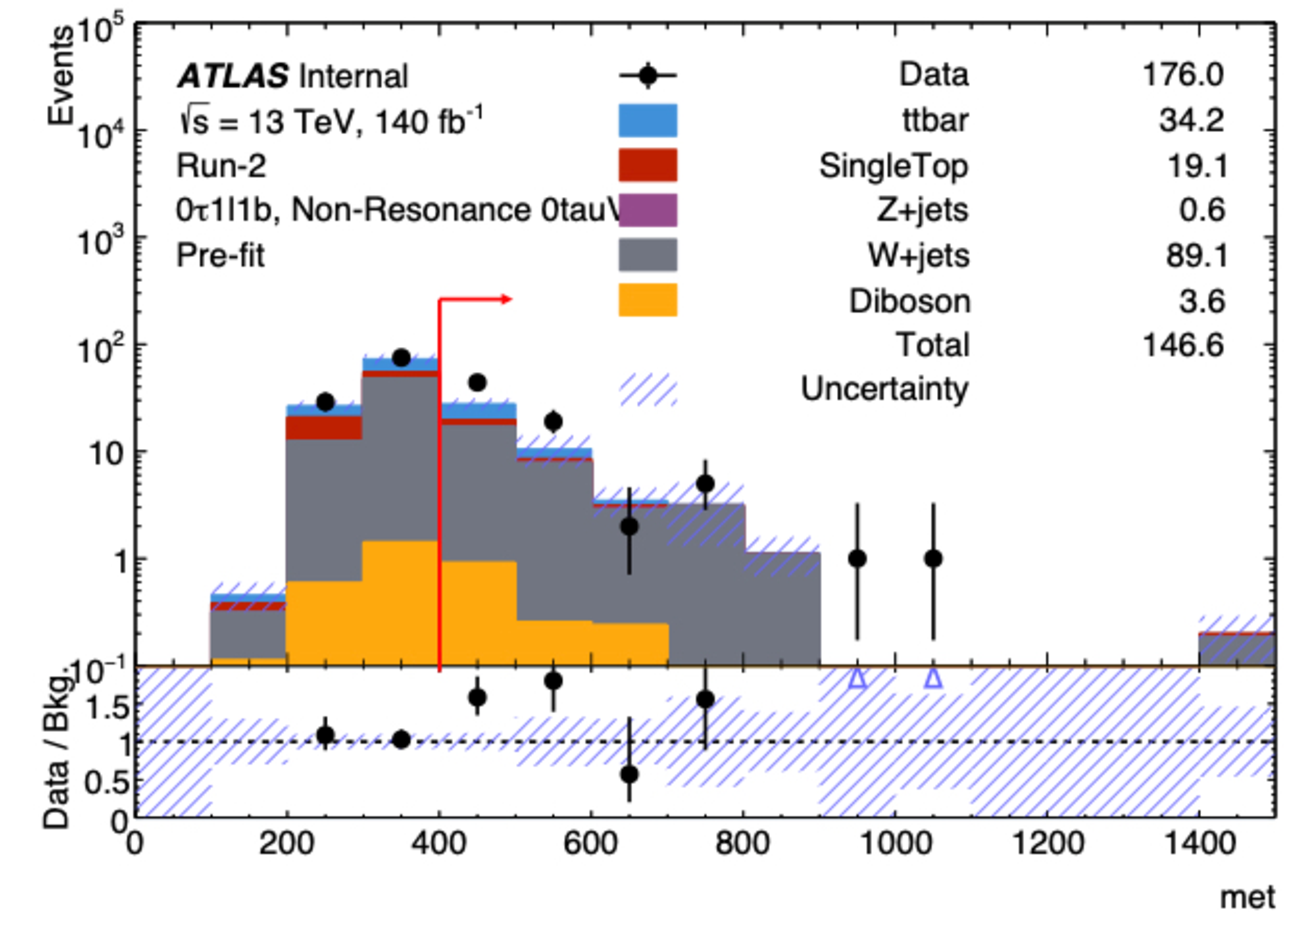
\includegraphics[width=\linewidth]{Figs/CH8/VRW_NonRes_met.pdf}
        \caption[]{$\met$}
    \end{subfigure}\hfill
    \begin{subfigure}{0.47\linewidth}
        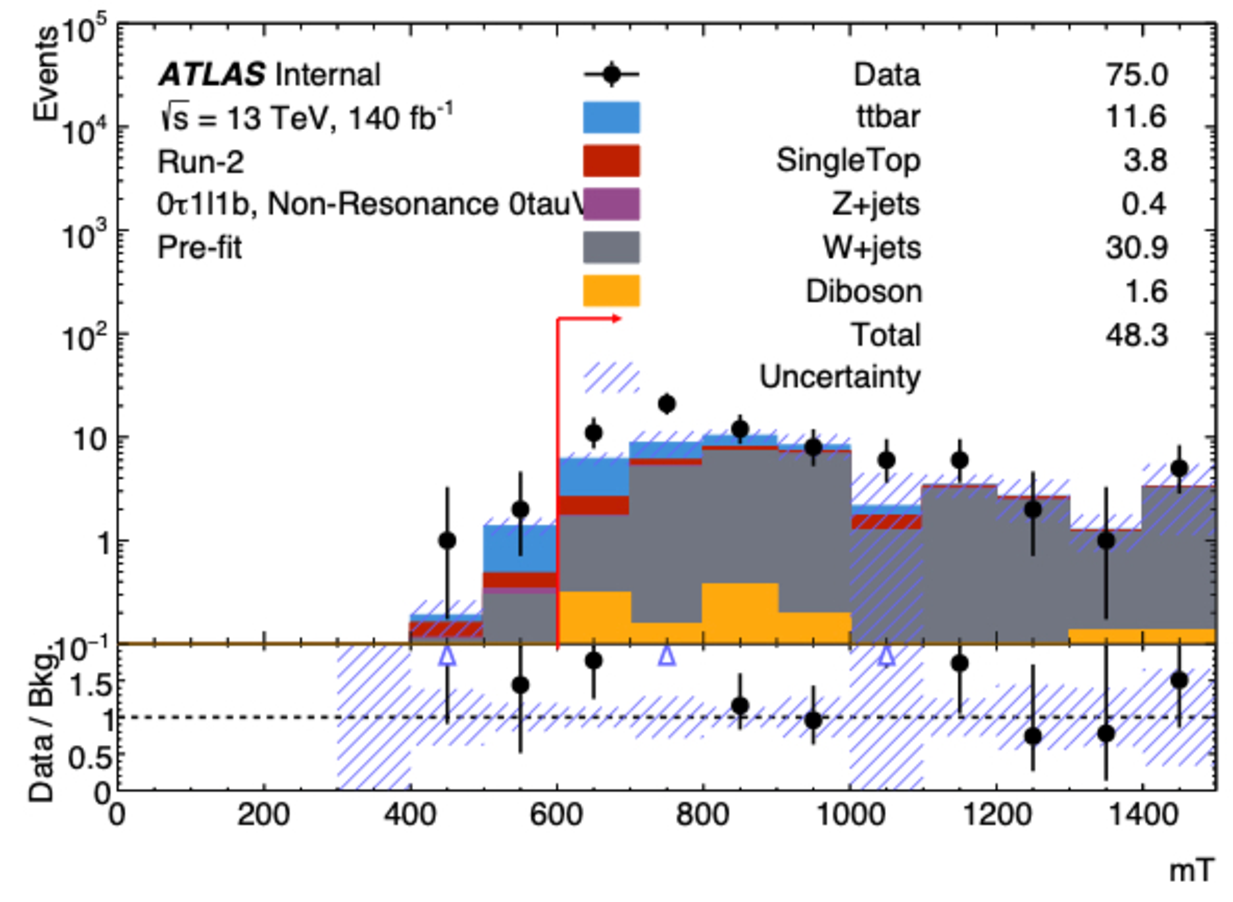
\includegraphics[width=\linewidth]{Figs/CH8/VRW_NonRes_mT.pdf}
        \caption[]{$\mT^\ell$}
    \end{subfigure}\par\medskip
    \begin{subfigure}{0.47\linewidth}
        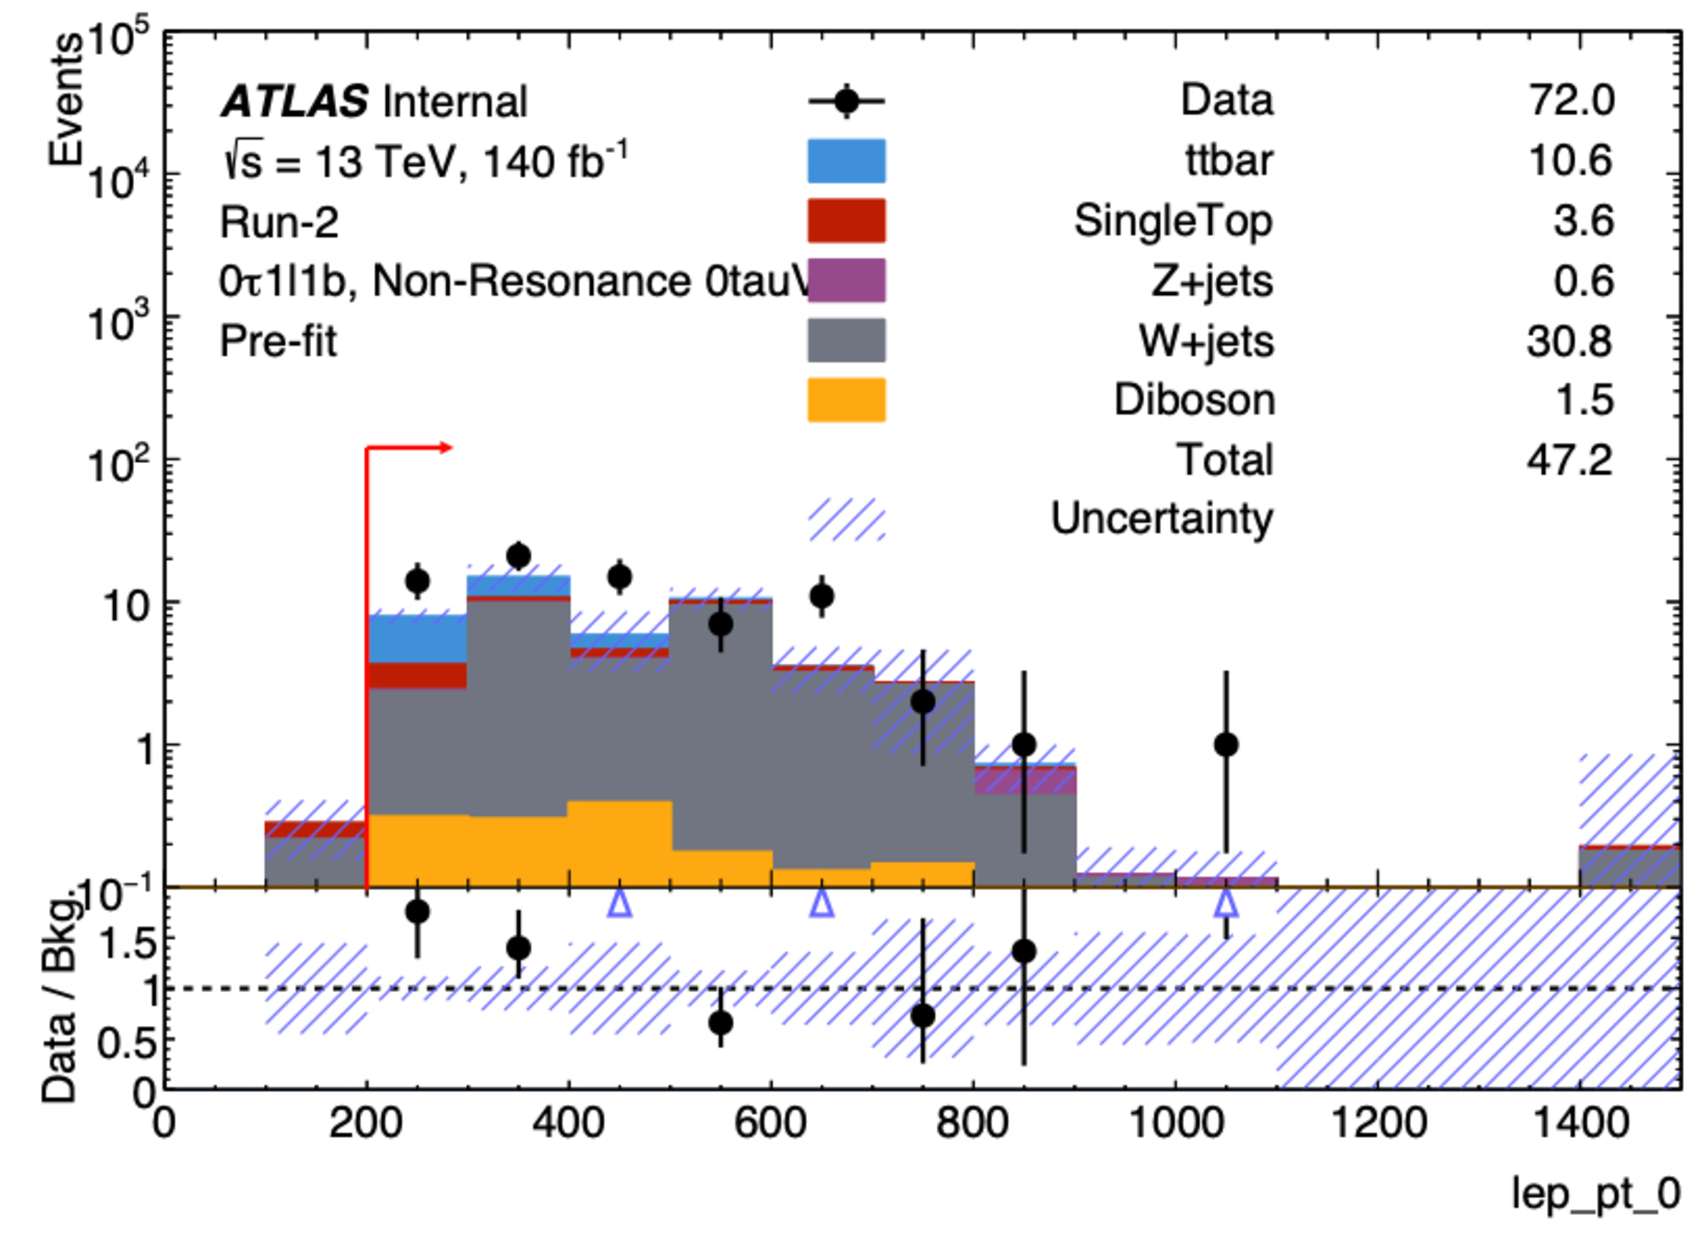
\includegraphics[width=\linewidth]{Figs/CH8/VRW_NonRes_lep_pT.pdf}
        \caption[]{$\pT^\ell$}
    \end{subfigure}\hfill
    \begin{subfigure}{0.47\linewidth}
        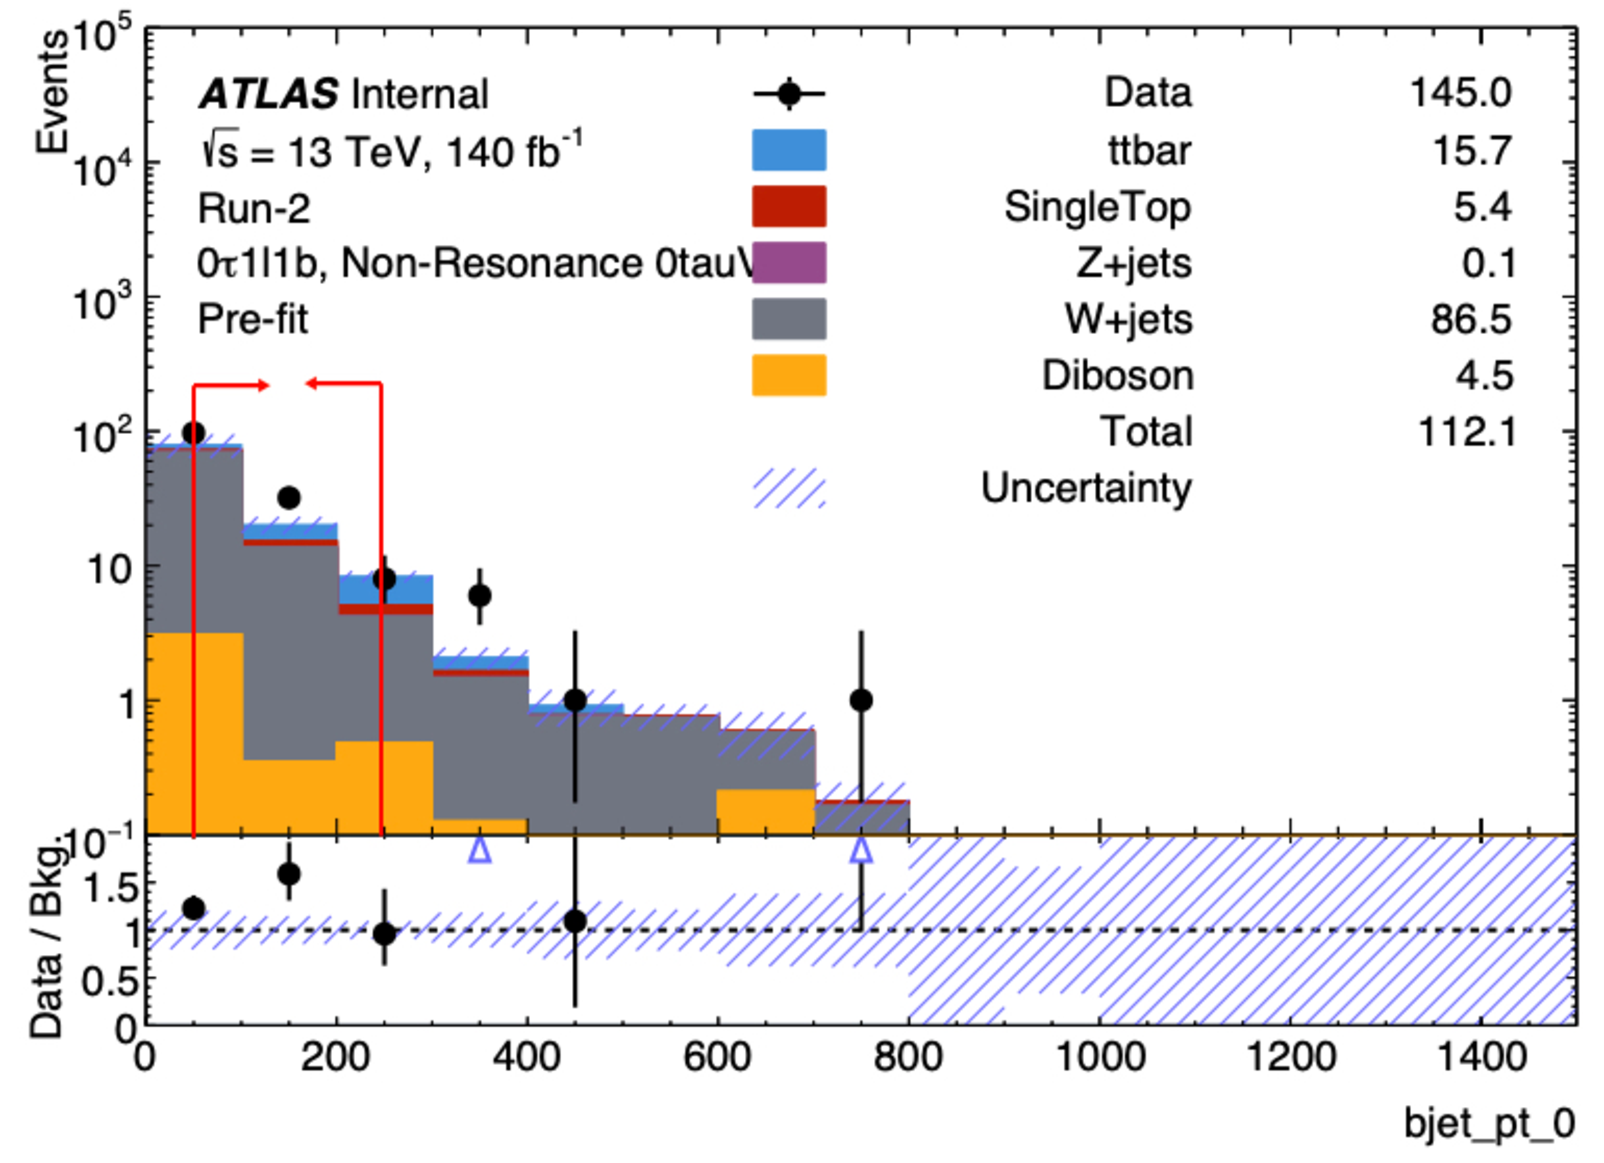
\includegraphics[width=\linewidth]{Figs/CH8/VRW_NonRes_b_pT.pdf}
        \caption[]{$\pT^b$}
    \end{subfigure}\par\medskip
    \begin{subfigure}{0.47\linewidth}
        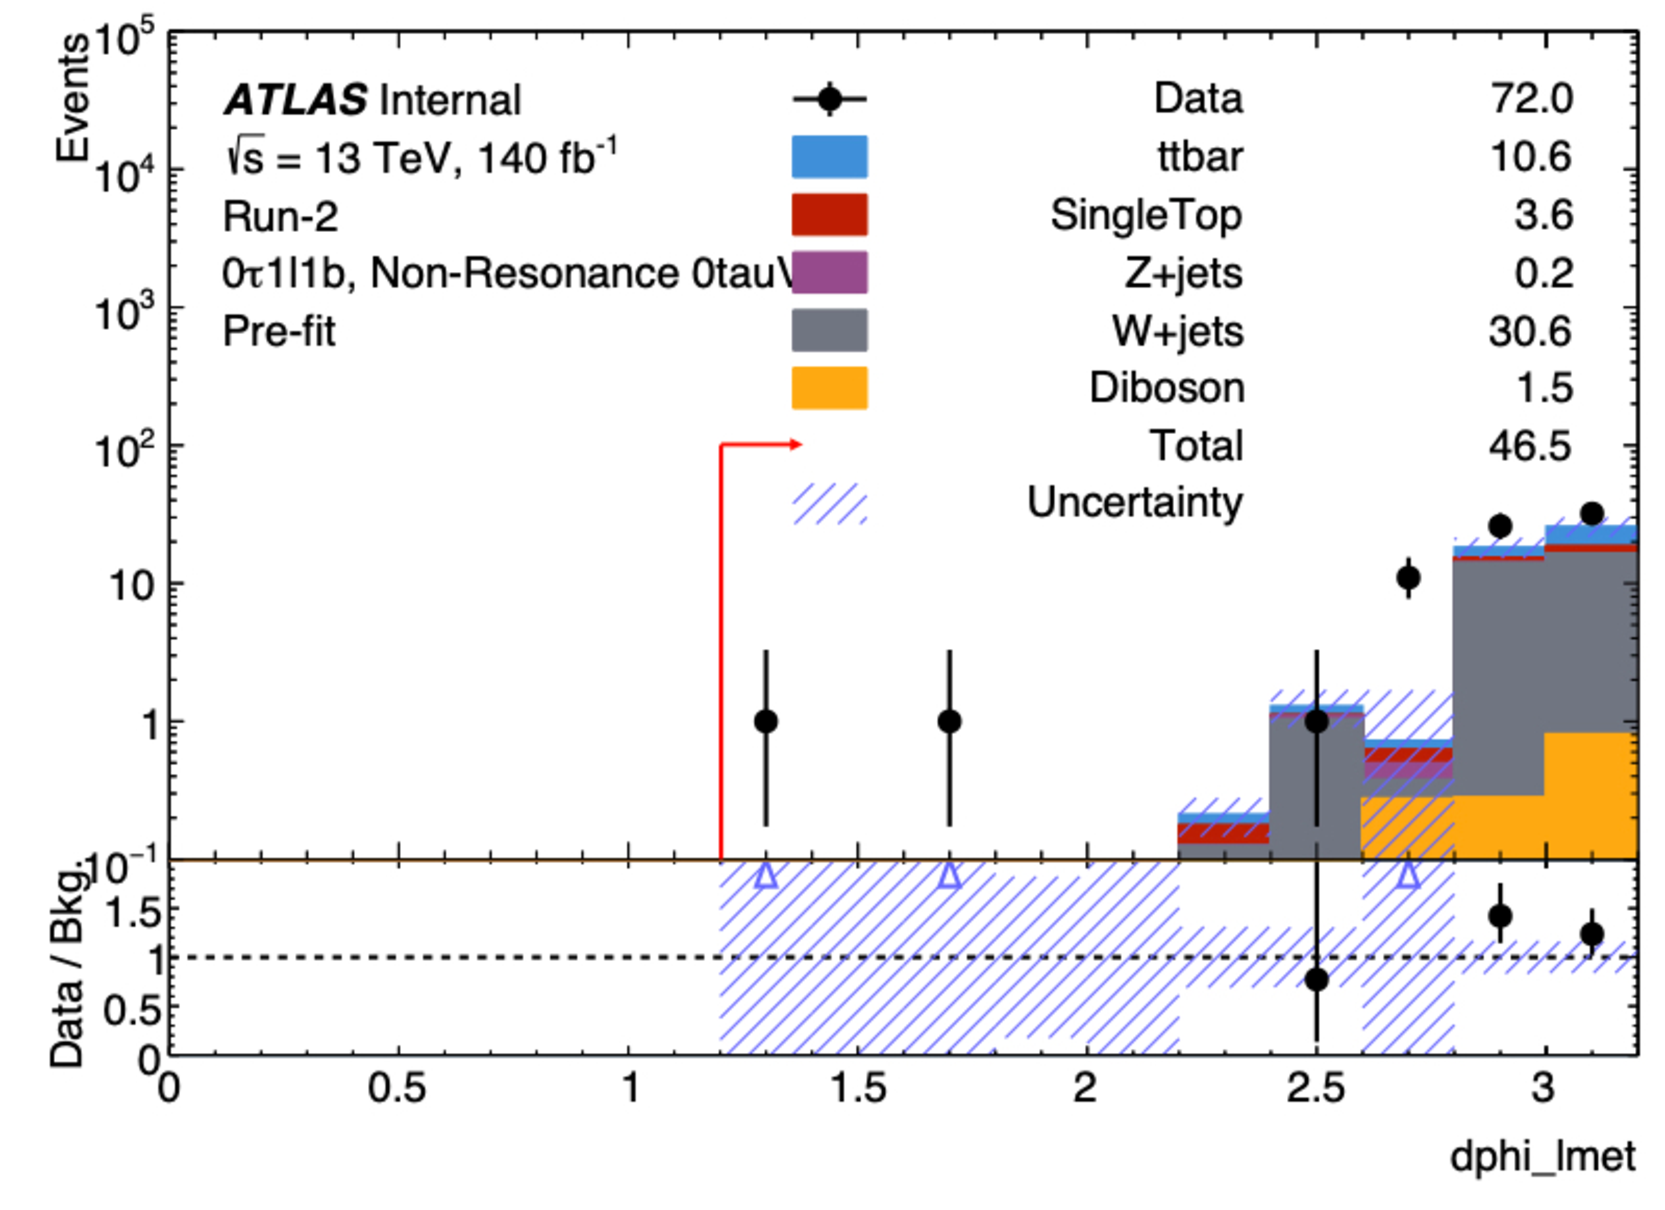
\includegraphics[width=\linewidth]{Figs/CH8/VRW_NonRes_DPhi.pdf}
        \caption[]{$\DphiLepMet$}
    \end{subfigure}\hfill
    \begin{subfigure}{0.47\linewidth}
        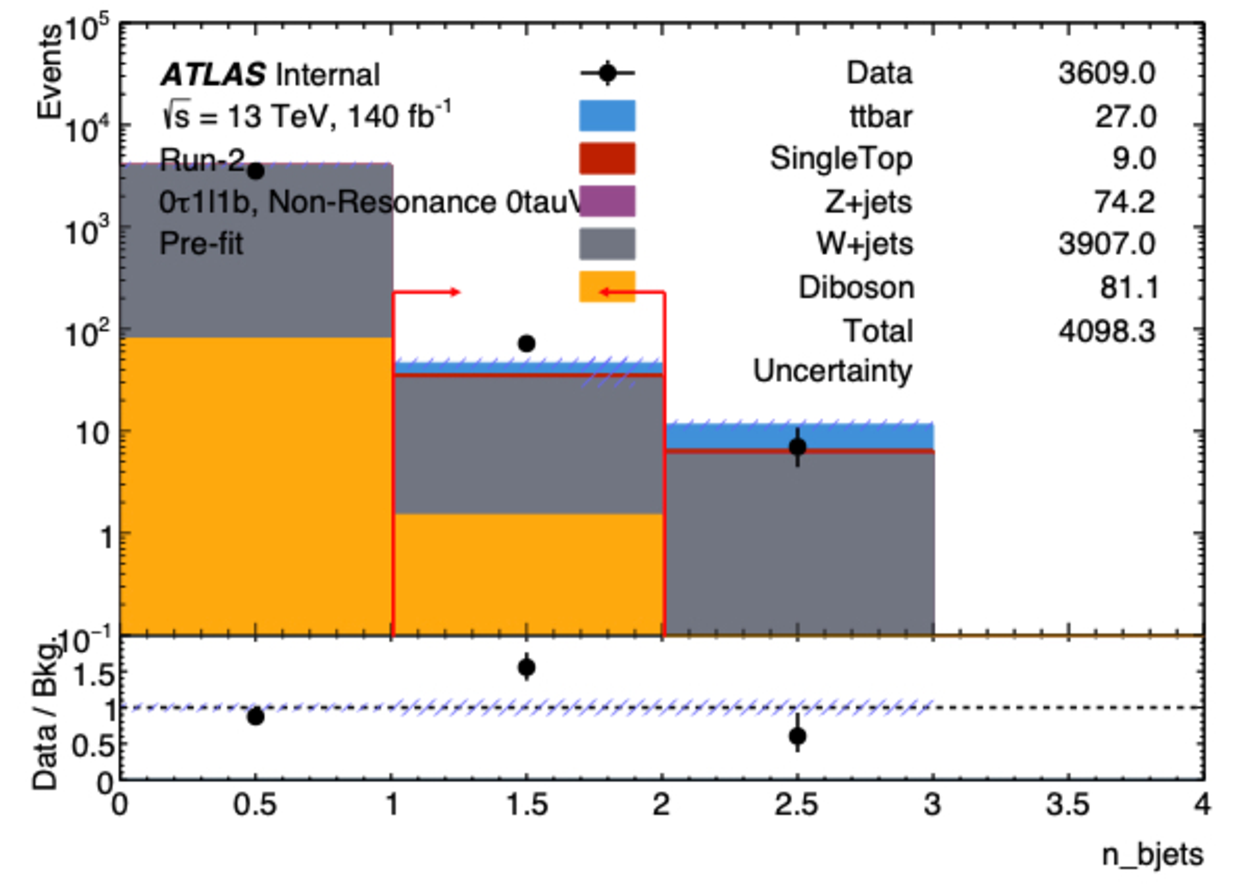
\includegraphics[width=\linewidth]{Figs/CH8/VRW_NonRes_nbjets.pdf}
        \caption[]{$N_b$}
    \end{subfigure}\par\medskip
    \caption[Pre-fit N-1 distributions in VRW-NonRes]{Pre-fit $N-1$ distributions in VRW-NonRes. The electron and muon channels are combined. The lower panels show data divided by the total simulated background. The hatched bands represent the statistical uncertainty in the prediction. The last bin includes the overflow. The original plot labels $0\tau$VR denote $\VRb$.}
    \label{fig:ch8_vrw_nonres}
\end{figure}
